%%
%% This is file `sample-manuscript.tex',
%% generated with the docstrip utility.
%%
%% The original source files were:
%%
%% samples.dtx  (with options: `manuscript')
%% 
%% IMPORTANT NOTICE:
%% 
%% For the copyright see the source file.
%% 
%% Any modified versions of this file must be renamed
%% with new filenames distinct from sample-manuscript.tex.
%% 
%% For distribution of the original source see the terms
%% for copying and modification in the file samples.dtx.
%% 
%% This generated file may be distributed as long as the
%% original source files, as listed above, are part of the
%% same distribution. (The sources need not necessarily be
%% in the same archive or directory.)
%% 
%%
%% Commands for TeXCount
%TC:macro \cite [option:text,text]
%TC:macro \citep [option:text,text]
%TC:macro \citet [option:text,text]
%TC:envir table 0 1
%TC:envir table* 0 1
%TC:envir tabular [ignore] word
%TC:envir displaymath 0 word
%TC:envir math 0 word
%TC:envir comment 0 0
%%
%%
%% The first command in your LaTeX source must be the \documentclass command.
\documentclass[manuscript,review,anonymous]{acmart}%%
%% \BibTeX command to typeset BibTeX logo in the docs
\AtBeginDocument{%
  \providecommand\BibTeX{{%
    \normalfont B\kern-0.5em{\scshape i\kern-0.25em b}\kern-0.8em\TeX}}}

%% Rights management information.  This information is sent to you
%% when you complete the rights form.  These commands have SAMPLE
%% values in them; it is your responsibility as an author to replace
%% the commands and values with those provided to you when you
%% complete the rights form.
\setcopyright{acmcopyright}
\copyrightyear{2018}
\acmYear{2018}
\acmDOI{10.1145/1122445.1122456}

%% These commands are for a PROCEEDINGS abstract or paper.
\acmConference[Woodstock '18]{Woodstock '18: ACM Symposium on Neural
  Gaze Detection}{June 03--05, 2018}{Woodstock, NY}
\acmBooktitle{Woodstock '18: ACM Symposium on Neural Gaze Detection,
  June 03--05, 2018, Woodstock, NY}
\acmPrice{15.00}
\acmISBN{978-1-4503-XXXX-X/18/06}


%%
%% Submission ID.
%% Use this when submitting an article to a sponsored event. You'll
%% receive a unique submission ID from the organizers
%% of the event, and this ID should be used as the parameter to this command.
%%\acmSubmissionID{123-A56-BU3}

%%
%% The majority of ACM publications use numbered citations and
%% references.  The command \citestyle{authoryear} switches to the
%% "author year" style.
%%
%% If you are preparing content for an event
%% sponsored by ACM SIGGRAPH, you must use the "author year" style of
%% citations and references.
%% Uncommenting
%% the next command will enable that style.
%%\citestyle{acmauthoryear}

%%
%% end of the preamble, start of the body of the document source.
\begin{document}

%%
%% The "title" command has an optional parameter,
%% allowing the author to define a "short title" to be used in page headers.
\title{A Blockchain Approach to Academic Assessment}

%%
%% The "author" command and its associated commands are used to define
%% the authors and their affiliations.
%% Of note is the shared affiliation of the first two authors, and the
%% "authornote" and "authornotemark" commands
%% used to denote shared contribution to the research.

\author{Sharareh Alipour}
\authornotemark[1]
\email{alipour@ipm.ir}
\affiliation{%
 \institution{School of computer science, Institute for research in fundamental sciences (IPM)}
 %\streetaddress{P.O. Box 1212}
 % \city{Dublin}
 % \state{Ohio}
% \country{USA}
% \postcode{43017-6221}
}

\author{Sina Elahimanesh}
\affiliation{%
 \institution{Department of computer engineering, Sharif university of technology}
 % \streetaddress{1 Th{\o}rv{\"a}ld Circle}
 % \city{Hekla}
 % \country{Iceland}
 }
%\email{larst@affiliation.org}

\author{Soroush Jahanzad}
\affiliation{%
 \institution{Department of computer engineering, Sharif university of technology}
 %\city{Rocquencourt}
 % \country{France}
}

\author{Parimehr Morassafar}
\affiliation{%
 \institution{Department of computer engineering, Sharif university of technology}
% \streetaddress{Rono-Hills}
% \city{Doimukh}
% \state{Arunachal Pradesh}
 %\country{India}
 }

\author{Seyed Parsa Neshaei}
\affiliation{%
 \institution{Department of computer engineering, Sharif university of technology}
% \streetaddress{30 Shuangqing Rd}
% \city{Haidian Qu}
 % \state{Beijing Shi}
% \country{China}
 }



%%
%% By default, the full list of authors will be used in the page
%% headers. Often, this list is too long, and will overlap
%% other information printed in the page headers. This command allows
%% the author to define a more concise list
%% of authors' names for this purpose.
\renewcommand{\shortauthors}{Alipour and et al.}

%%
%% The abstract is a short summary of the work to be presented in the
%% article.
\begin{abstract}
In this paper, we propose a novel method for academic assessment inspired by the decentralized applications made possible by blockchain technology.
  The proposed method applies to a wide range of academic material, including assignments, exams, academic papers, etc  
  and tackles issues regarding potential personal bias and makes assessment possible without the need to rely on a few assessors.
  We examine the challenges and possibilities that arise with this method and further explore more general applications in areas such as education.
  In the experiments conducted for this research, poll results show generally positive views toward the fairness of this system compared to the traditional methods.

\end{abstract}

%%
%% The code below is generated by the tool at http://dl.acm.org/ccs.cfm.
%% Please copy and paste the code instead of the example below.
%%
\begin{CCSXML}
<ccs2012>

<concept>
<concept_id>10003120.10003121.10003122</concept_id>
<concept_desc>Human-centered computing~HCI design and evaluation methods</concept_desc>
<concept_significance>500</concept_significance>
</concept>
<concept>
<concept_id>10002944.10011123.10011673</concept_id>
<concept_desc>General and reference~Design</concept_desc>
<concept_significance>300</concept_significance>
</concept>
<concept>
<concept_id>10002944.10011123.10011131</concept_id>
<concept_desc>General and reference~Experimentation</concept_desc>
<concept_significance>300</concept_significance>
</concept>
<concept>
<concept_id>10011007.10011074</concept_id>
<concept_desc>Software and its engineering~Software creation and management</concept_desc>
<concept_significance>300</concept_significance>
</concept>
<concept>
<concept_id>10010405.10010489</concept_id>
<concept_desc>Applied computing~Education</concept_desc>
<concept_significance>500</concept_significance>
</concept>
</ccs2012>
\end{CCSXML}

\ccsdesc[500]{Human-centered computing~HCI design and evaluation methods}
\ccsdesc[300]{General and reference~Design}
\ccsdesc[300]{General and reference~Experimentation}
\ccsdesc[300]{Software and its engineering~Software creation and management}
\ccsdesc[500]{Applied computing~Education}

%%
%% Keywords. The author(s) should pick words that accurately describe
%% the work being presented. Separate the keywords with commas.
\keywords{ Blockchain design, Assessment, Education}


%%
%% This command processes the author and affiliation and title
%% information and builds the first part of the formatted document.
\maketitle

\section{Introduction}



A blockchain is a growing list of records, called blocks, that are linked using cryptography.
% Each block contains a cryptographic hash of the previous block, a timestamp, and the transaction data.
Blockchain is the fourth industrial revolution that came after the inventions of the steam engine, electricity, and information technology. Blockchain technology is expected to revolutionize the operating modes of commerce, industry, and education, as well as to promote the rapid development of a knowledge-based economy on a global scale. Due to its immutability, transparency, and trustworthiness for all transactions executed in a blockchain network, this innovative technology has many potential applications. 
Blockchain is a foundational technology that documents transactions in a decentralized, secure, transparent, and immutable way and has a major impact on
design and implementation of digital business processes in many application areas such as the internet of things, smart grid, supply chain, finance, or notarization \cite{ian,nar}.


In this paper, our focus is on applications of blockchain technology in education and particularly in academic assessments. The main concern in assessment is fairness.
A blockchain is decentralized and it can guarantee transparency and fairness. 
So, we propose a peer-to-peer grading mechanism using blockchain technology. We need to consider the challenges and issues that might happen. We 
discuss possible issues and try to find a way to overcome each of them.
We also implemented our idea and did some experiments on homework assessment in a real class and present our results.

 

\subsection{Related works}

The blockchain was first introduced by Satoshi Nakamoto in 2008. In his famous ``white paper" \cite{nak}, Nakamoto introduced a decentralized transaction ledger for the cryptocurrency bitcoin as the first application of blockchain.
%This disruptive technology will have a significant impact on national governance, institutional functions, business operations, education, and our daily lives in the $21$st century. It has the potential to transform the current Internet from ``The Internet of Information Sharing" to ``The Internet of Value Exchange".
During the initial stages of its appearance, blockchain technology was not able to draw a lot of attention. However, as bitcoin continues to run safely and steadily over the years, society has since become aware of the enormous potential applications of the underlying technology of this invention is not only in cryptocurrency but also in many other areas. Blockchain technology has become a hot topic for more and more countries, institutions, enterprises, and researchers.


It has been argued that there is a unique role for the HCI community in linking the design and application of blockchain technology towards lived
experience and the articulation of human values \cite{els}. Detailed mapping and examination of
emerging applications of blockchain technologies, in an
effort to chart the space for the HCI community, is presented in \cite{els}.
The research in HCI concerning blockchain is mostly built on a history of
work in HCI on money, finance, and peer-to-peer exchange \cite{bel, car, fer, kay,lam, mil,shi} but largely concerns the
experience, motivations, and values of Bitcoin users. For more information on blockchain applications in HCI see \cite{els}, where a typology of emerging blockchain applications is constructed.


Nowadays, some universities and institutes have applied blockchain technology in their educational system, and most of them use it to support academic degree management and digital transformation of certification processes. The blockchain for educational platforms represents paper certificates as digital certificates and their fingerprints (unique hashes) are written on the blockchain. In addition, the identities of certification authorities and certifiers are also stored in the blockchain. Finally, smart contracts support the management of certification authorities and certifiers as well as monitoring or revocation of certificates.
The University of Nicosia\footnote{http://www.educationmalta.org/blockcerts-to-be-developed-in-malta/} and the MIT Media Lab Learning\footnote{https://certificates.media.mit.edu/} are examples of the institutions that work on using blockchain in issuing digital certificates.
See \cite{chen} and \cite{gra} for more examples.


Likewise, in the context of education, the blockchain can formulate the whole transcript. In the formal learning context, this includes learning contents and outcomes as well as students' achievements and academic certificates. Subsequently, in the informal learning context, information about research experience, skills, online learning experience as well as individual interests are included. These data can be safely stored and accessed on a blockchain network in appropriate ways.
Blockchain technology can also contribute to the reduction of degree frauds. In the past, numerous cases of fraudulent degrees were reported. However, this can be avoided by employing blockchain in granting and managing the students' degrees. Miners from all over the world match the data with the users' IDs and store them in the blockchain, and subsequently check, validate, and maintain the data. The blockchain distributed ledger is immutable and trustworthy. Thus, reliability and authority are both ensured, which will significantly reduce fraud.

Blockchain can be used as a ``capacity-currency transformation bank'' \cite{chen}. Specifically, the blockchain learning ledger records detailed information about the users' learning experience and follows the development of their knowledge and skills. All of them can be transformed into a sort of digital currency and stored on a blockchain network according to a series of comprehensive standards. Students will gain rewards through their efforts on studies, which is called ``learning is earning'' \cite{sharp1}. Some schools have also started the application with this concept, for example, \cite{sharp1} claimed a kind of Education Reputation Currency named Kudos. It can be used to measure learning outcomes and stored in a virtual wallet.

We believe that blockchain technology has a lot more potential in education than these and it can solve many issues in educational systems.
In this paper, we propose a new method for the assessment of educational materials. We implement our idea and do some experiments in real classes.



\section{Why blockchain?}
Blockchain as new technology can play an important role in education.
In this age, educational policies focus on collaboration, creativity, content creation, and digital literacies \cite{khar}.
In parallel, educational technology innovation is increasingly moving beyond traditional software and hardware tools to include technologies such as augmented and virtual reality \cite{9459415},
social media, tangibles, robotics, AI, and one of the newest technologies, blockchain.
So, there are important subjects to consider such as\cite{khar}; The challenges of evaluating
the impact of deploying innovative technologies in
the classroom; Find the best practices, strategies,
methods and tools to support the deployment and
the evaluation process of such technologies in the
classroom; Outline the logistical, ethical and
social (i.e., non-methodological) challenges that
are associated with such technologies (e.g. the
use of social media in the classroom), of which
researchers need to be aware when designing,
deploying and evaluating such technologies in the
classroom.

In the traditional assessment method, the teacher or teaching assistants assess the homework and exams. Some issues happen in this procedure, which we explain in the following.
The main concern for teachers and students is fairness. Since the system is centralized and controlled by only a few people (the teacher and teaching assistants), there is always a possibility that a teacher or teaching assistants have mistakes in assessments, and the procedure might be unclear and biased.
Also, the teacher might have time limits. For a teacher or teaching assistant that assesses homework, this might be a boring job. Sometimes the teacher or teaching assistant might not have enough accuracy or might have a problem with a specific student which affects assessments.
So, our goal is to propose a new assessment method with the following properties.
\begin{itemize}
\item Decentralize the process. 
\item Ensure transparency. 
\item Have a universal and clear procedure. 
\item Extensive peer-review. 
\item Faster results.
\item Reliable infrastructure.
\end{itemize}

An assessment system with these properties can satisfy both students and teachers. We want to define our system based on the blockchain since a blockchain is decentralized and it can guarantee transparency and fairness.


\section{Our proposed blockchain}
In this section, we introduce a blockchain for homework assessment.
In our proposed blockchain students submit their homework anonymously. Now it is time to assess the homework. In our blockchain, all students of a class can assess the homework anonymously.
The students, the teacher, and the teaching assistants compete to assess the submitted homework. After assessing the homework, they release the papers, the details of the assessment, and the given grade as a block to the blockchain. Their knowledge score in the system and the time of their assessment determine the priority and impact of that block and the rewards they receive.
  The students get a small amount of score for assessing each paper. Each homework should be assessed by at least three (can vary) students. Now the students act as miners and check the assessments details of papers and add the verified assessments to the blockchain. Each block consists of homework/exam, responses, and grading results. The miners get a score (similar to the bitcoin in the bitcoin blockchain) for verifying the grades. So, the winner is not who possesses better hardware, but who knows more of the course.
To ensure this, every student gives a score to the student that assessed her paper 
so that the blocks associated with students who have higher assessment scores can have a higher chance to be accepted.
See Fig. \ref{fig1} for a simple chart of the proposed blockchain.


As far as we know the idea of our proposed blockchain is new and unprecedented, so we consider some policies before implementing it. For example, the system should have a good abstraction since users may not have a blockchain technology background. Who revises the grades should not be the person who graded in the first place. Each paper might be graded multiple times to find and correct errors. Details of grading should be included in the block. Students should be able to consult the instructor when needed.


The possible problems in the proposed system that might come to mind for the first vision are the following and we explain why the system works by adding 
extra policies to prevent these problems.
\begin{itemize}
\item Fake users: users are rated and validated by score.
\item Biased scores: other users validate previous scores. 
\item Lack of checkers and correctors: users are motivated by reward scores.
\item Other problems in common with bitcoin: will work out the same way it did for Bitcoin.
\end{itemize}

Note that in our system each paper can be assessed and verified multiple times since we want to have a more reliable score and give a chance of collecting rewards to the weaker students. However, after the first three assessments of a paper are done, the assessment reward decreases.
The appropriate amount of the score for assessment and verifying can be determined experimentally according to the opinions of the students and teacher. 


\begin{figure}[H]
 \caption{A simple chart of the proposed blockchain.}

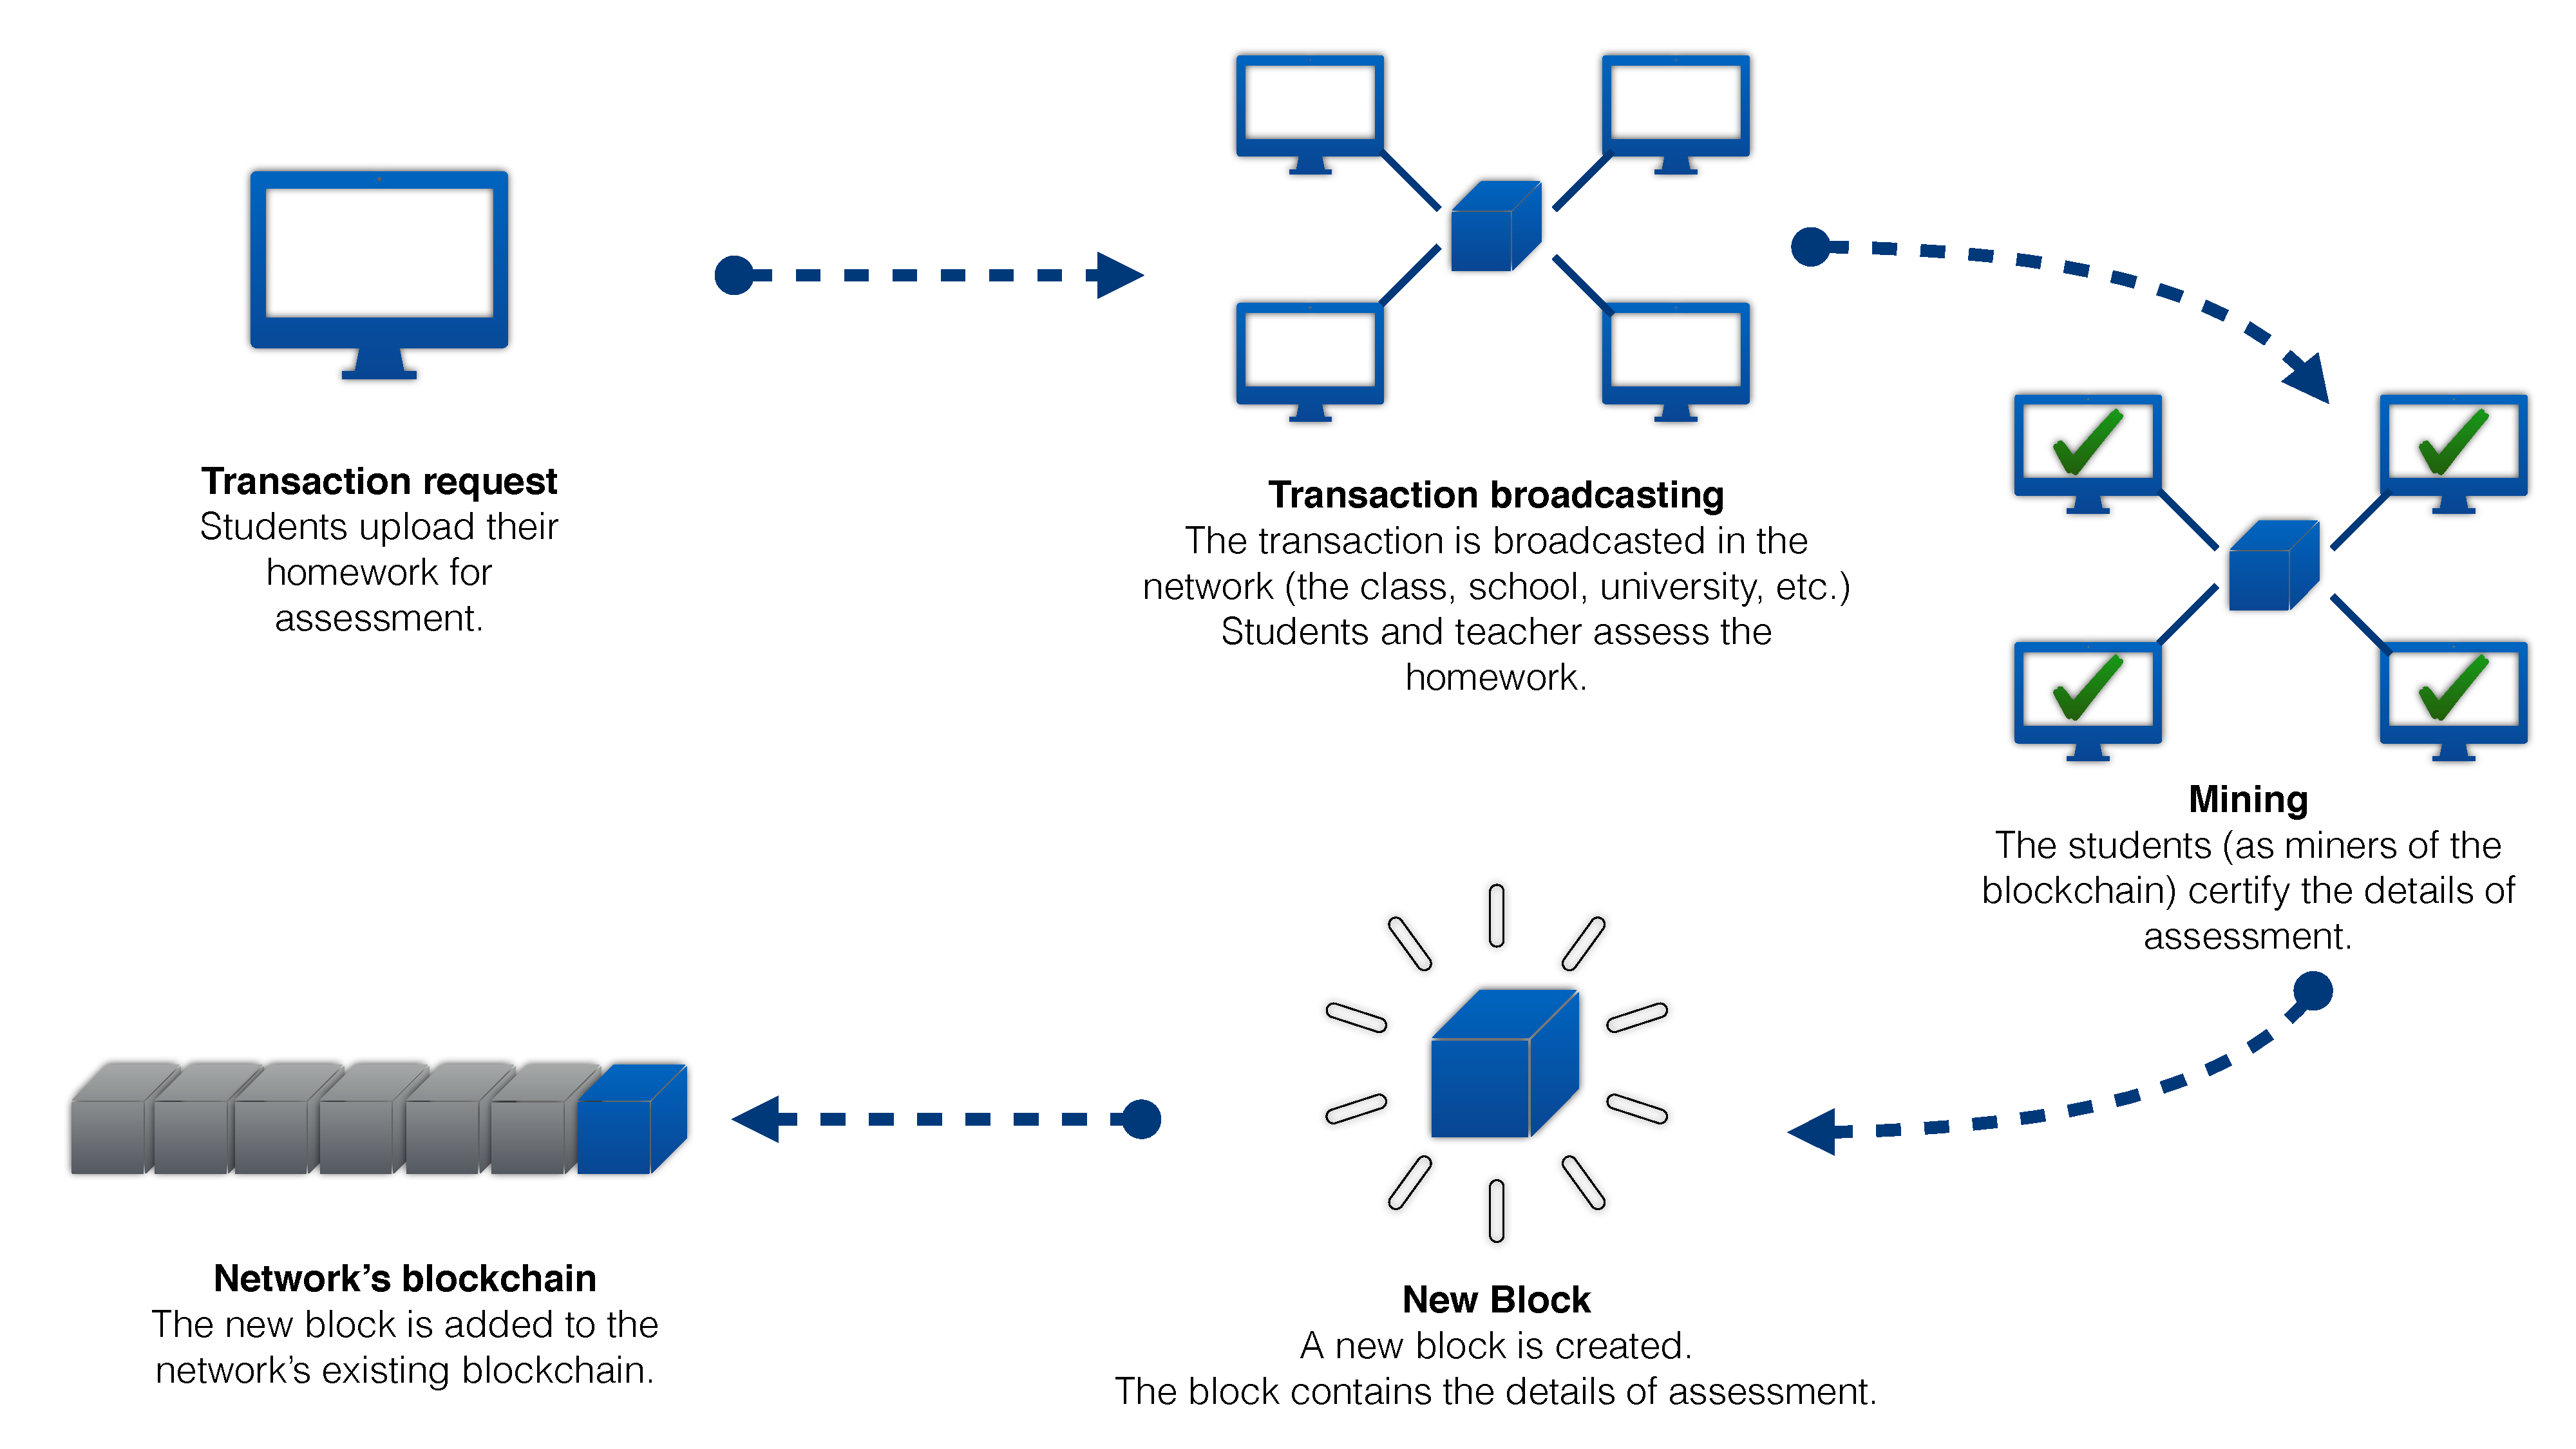
\includegraphics[scale=0.15]{fig1.pdf}


\label{fig1}
\end{figure}



\section{Implementation}

Based on our research we decided to implement the system in a half-centralized model to perform the experiments. 
We designed a website where students were able to upload their homework and download the homework of other students for assessment. After an assessment, they could upload the grades and details of the assessment and the score of assessment of each assessor. They also have access to all the materials including the details of assessments and the score of each assessor (of course, the assessors were anonymous).

In our experimental results
the students and teacher work in a decentralized setting but we have access to all the data and the admin can manipulate the system. This is against the philosophy of blockchain. But note that as the admin, we just observe the behavior of the students and the teacher in this setting which is in a decentralized setting.
We need the observation to choose or design the best blockchain platform for our system in the future. In our initial experiments, our goal is to implement our idea and see how it works, improve the system and solve the possible issues. In the next steps, we will design a real decentralized system based on our experimental results and the feedback from the users. 
Fig. \ref{fig2} presents the main functionalities in our proposed system.
\begin{figure}[H]
 \caption{Main functionalities of our system}
 
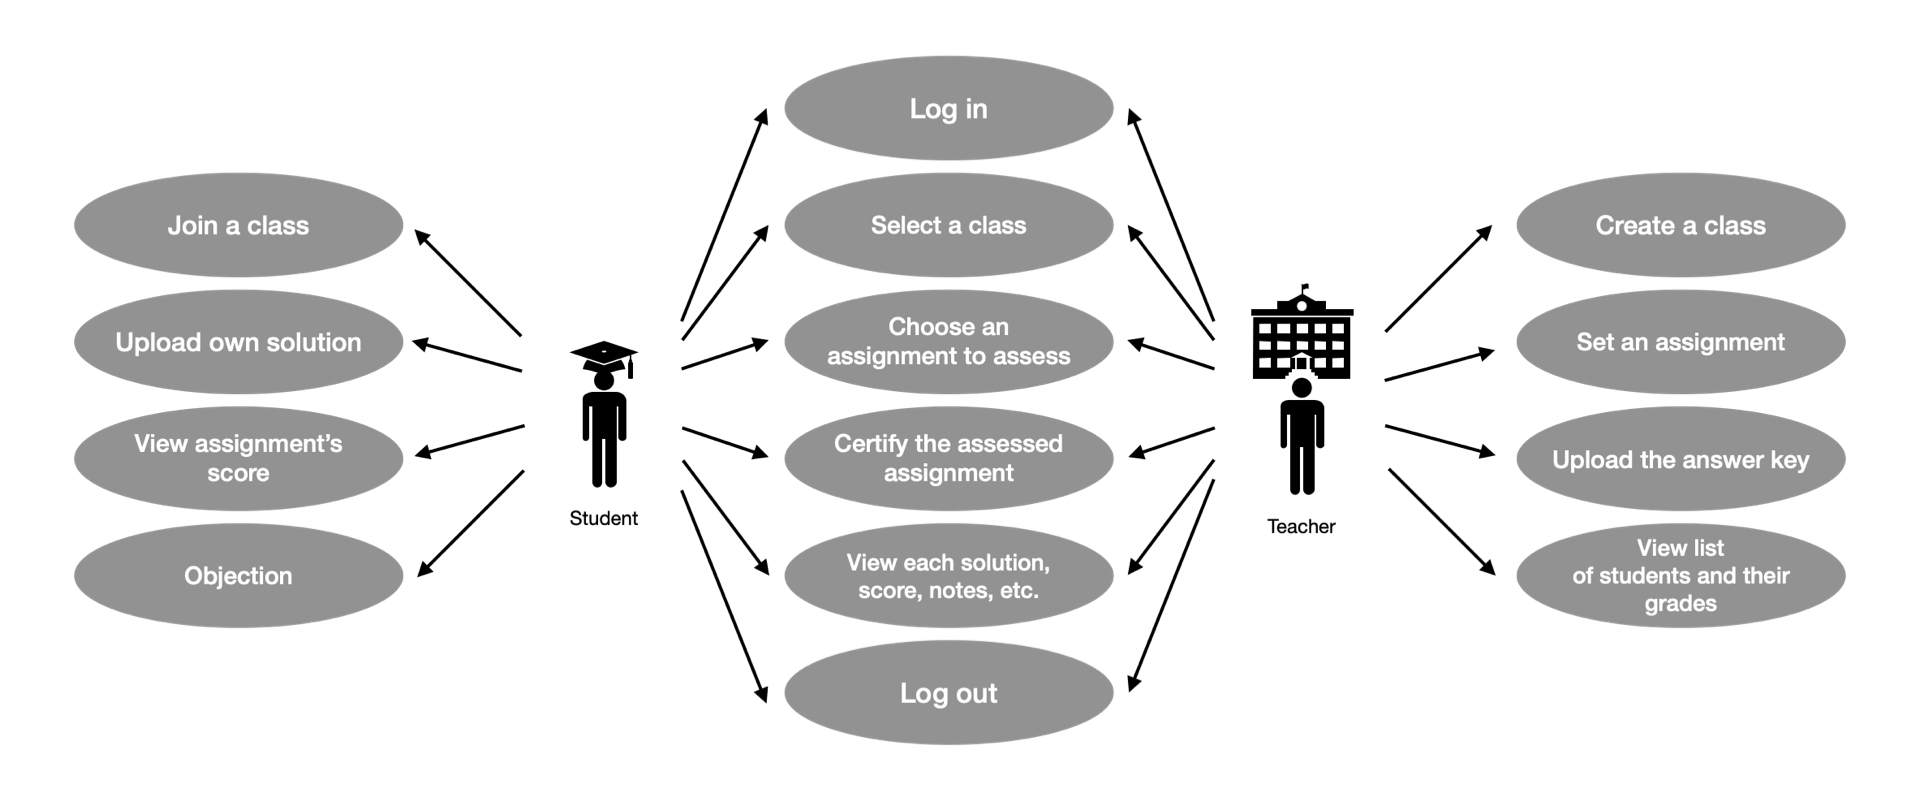
\includegraphics[scale=0.15]{fig2.jpeg}


\label{fig2}
\end{figure}

\subsection{Our experiment}

As an initial experiment, about fifty students (two classes) from the undergraduate level assessed their first homework. Each homework was assessed by three students. We gave eight hours to the student for completing this task. In the end, we released their final grade. Eighty percent of the final grade came from the mean of the grades given by the students and
the remaining twenty percent was given based on the quality of assessments done by each student, determined by asking each student about the fairness of each assessment done on their paper. Note that the identity of the assessors was not known by the students.
This twenty percent helped the people who were unable to submit their homework by the deadline. They had the chance to attend the assessment process and get twenty percent of the grade.
We also took the grades through the traditional method into consideration.
Next, we asked the students to give a score from zero to ten to some questions about the fairness and speed of the proposed method and the traditional method. See Table \ref{t1} for the average scores given by students.


\begin{table*}[h!]
\caption{The questions and the averages of scores given by the students.}
\begin{center}
\begin{tabular}{| l | ll |}
 \hline
 Question & Average in this method & Average in the traditional method\\ \hline
 Fairness of your grade& 8.49/10& 7.89/10 \\ \hline
 
 Fairness of overall grades of the students &8.13/10 &7.38/10 \\ \hline
 
 Grading speed & 7.76/10 & 5.44/10 \\ \hline
 
 
 
 \end{tabular}
\end{center}
\label{t1}
\end{table*}



We also asked the participants to choose one of the methods and roughly 60 percent of them preferred the new method.
The average time for assessing the papers per student was 1.31 hours.
So as we expected, this method was faster and fairer according to the students' opinions.

We also asked the students to give their comments and suggestions to improve the performance of our model in the future.
Here are some feedbacks. 
The suggestions and comments are worthy of consideration in future developments. However, the complaints are not as troublesome as they seem, and we explain why.
\begin{itemize}
\item What happens if all of the students in the class decide to give a full grade to each other?

This does not seem to be a problem because the students value their efforts and know it would not be fair to give everyone a full score.
The multiple evaluations of scores and the presence of the teachers and teaching assistants in the process also ensure the authenticity of the given scores.

\item The students of the class do not have enough knowledge.

In standard homework, there are always people who can achieve the perfect score. 
In the case that there is exceptionally hard homework or one without a clear answer, the stronger students, teaching assistants, or the teacher can release the answers and the scoring guide.
Note that in most cases students can tell the right answer apart from the wrong one, even if they don't know the answer. So
because the students can see the details of all the corrected papers, they can assess the papers correctly.

\item The students can not have any objections.

Unfortunately, we did not have the option to verify the scores in our experiment, but in our proposed blockchain it seems that no one will have an objection since each homework is assessed at least three times and is verified by the students and the miners to be fair and correct.



\end{itemize} 
In conclusion, we believe that with some additional properties and a few modifications, this system is going to be preferred by a large portion of the students.
Some suggestions might be considered for future experiments, for example, for more accuracy, the teacher can release the solutions after the deadline of the homework or the exam and in the assessment process, students can have an option to skip the questions and solutions that are not clear for them or the questions which they don't know the exact answer to.
Note that by doing more experiments, we can improve the performance of the system, since the feedbacks, suggestions, and comments help us to resolve the existing problems and deal with the challenges.
\section{Advantages and challenges of our proposed Blockchain and further applications}

Fairness and accuracy in grading: Since each paper is graded by at least three people and the details of grading are available in the blockchain, the grading system is decentralized and by the proposed method the chance of any issue being present is low.

Time-saving: In our system, the papers are graded by the students of the class so it saves the teacher's or teaching assistants' time. Also by this method, students get their grades sooner than the classic method. 

Learning: Students of the class learn much by assessing their homework. For example, since the graded papers are available in the blockchain, the weaker students can use the graded papers in the blockchain to correct the remaining pieces of homework.

There are also some challenges we face. This blockchain in its first version is used only for homework assessment. However, assessing the exams is more challenging and this might cause some issues. In the future, we will try to improve the policies to overcome the challenges of exam assessment.
Students should put time into the assessment of the papers. It might benefit the process to reduce the number of homework to make the students happier and eager to learn through assessment of other's papers as well.
 Every new system needs time to settle down. So at first the teachers and students might not accept this system. However, we can try to improve it and make it more user-friendly. We should provide more detailed information about our method and its benefits to the participants. In our experiment, the students were not fully aware of the details and they had some doubts which might have affected their answers to our questions.



 \subsection{Another application: taking a course on blockchain}
 
 Our experiments show that the proposed blockchain results in an acceptable and reasonable system that provides a fairer environment for academic assessment.
 As a result, we can use the idea for other similar applications too. In this proposed blockchain, our goal was to decentralize the process of assessing the academic materials.
 To extend this idea, we can think of a complete ecosystem of taking courses available on a blockchain.
 Suppose that a group of people decide to study a book or get a course together. They can have a teacher, study together, or watch the online courses to learn.
 In the absence of a qualified teacher or the lack of any educational support other than teaching, a blockchain can be beneficial. 
 We are going to propose a blockchain to support students through the learning process and issue a certificate for the work that they do.
 In this blockchain, people begin to learn the desired subject, and throughout the process, they design problem sets and ask others to answer the questions.
 After solving the problems designed by other learners, they assess each other's works like the method proposed in this paper.
 For example, Alice can ask Bob to examine her knowledge and assess her works. 
 Since everything (questions, answers, grades, detail of assessment, $\dots$.) is available on the blockchain, other people (including Bob) can check everything.
 It is worth noting that students are not aware of each other's identities, which results in organic fraud detection i.e. anything about a person can be examined in this system, leaving no doubt.
 Upon completion of a course, the attendees will get a certificate if they have eligible grades. Note that this is just an idea and it probably can not replace the traditional system in this exact form.
 However, the reliability, availability, and performance of such an ecosystem appear to be potentially much more than current online course platforms like Coursera.

\bibliographystyle{ACM-Reference-Format}
\bibliography{sample}



\end{document}




%%
%% If your work has an appendix, this is the place to put it.
\\endinput
%%
%% End of file `sample-manuscript.tex'.
